\subsection{Ethylene combustion in a perfectly stirred reactor}
The PSR model of Omnisoot\footnote{\href{https://github.com/mohammadadib-cu/omnisoot-cv/tree/main/examples/psr_pfr}{https://github.com/mohammadadib-cu/omnisoot-cv/tree/main/examples/psr\_pfr}} was used to simulate ethylene combustion at different equivalence ratios, $\phi = 1.9$, 2.0, and 2.1 in a perfectly stirred reactor connected to a flow reactor~\citep{manzello2007soot}. PSD measurements were conducted at the end of the flow reactor using a Nano-Differential Mobility Analyzer (Nano-DMA). The volume ($V$) and nominal residence time ($\tau_{psr}$) of the PSR are 250~ml and 11~ms, respectively~\citep{manzello2007soot}. The flow reactor is 70~cm long with an inner diameter of 5.1~cm. The reactants enter the adiabatic PSR at 300~K with an inlet mass flow rate of $\dot{m}_{in} = \rho V / \tau_{psr}$, where $\rho$ was calculated at the reactor temperature of 1723~K~\citep{lenhert2009effects}. The PSR simulation was continued until a steady-state condition was reached for all the solution variables. The final gas composition, temperature, and soot properties from the PSR were used as inlet conditions for the PFR simulations, yielding an average axial velocity of 14.5~m/s in the PFR, which is consistent with the values reported in~\citep{manzello2007soot}.


\begin{figure*}[!t]
	\centering
	\begin{tikzpicture}
		\draw (0, 0) node[inner sep=0] 	{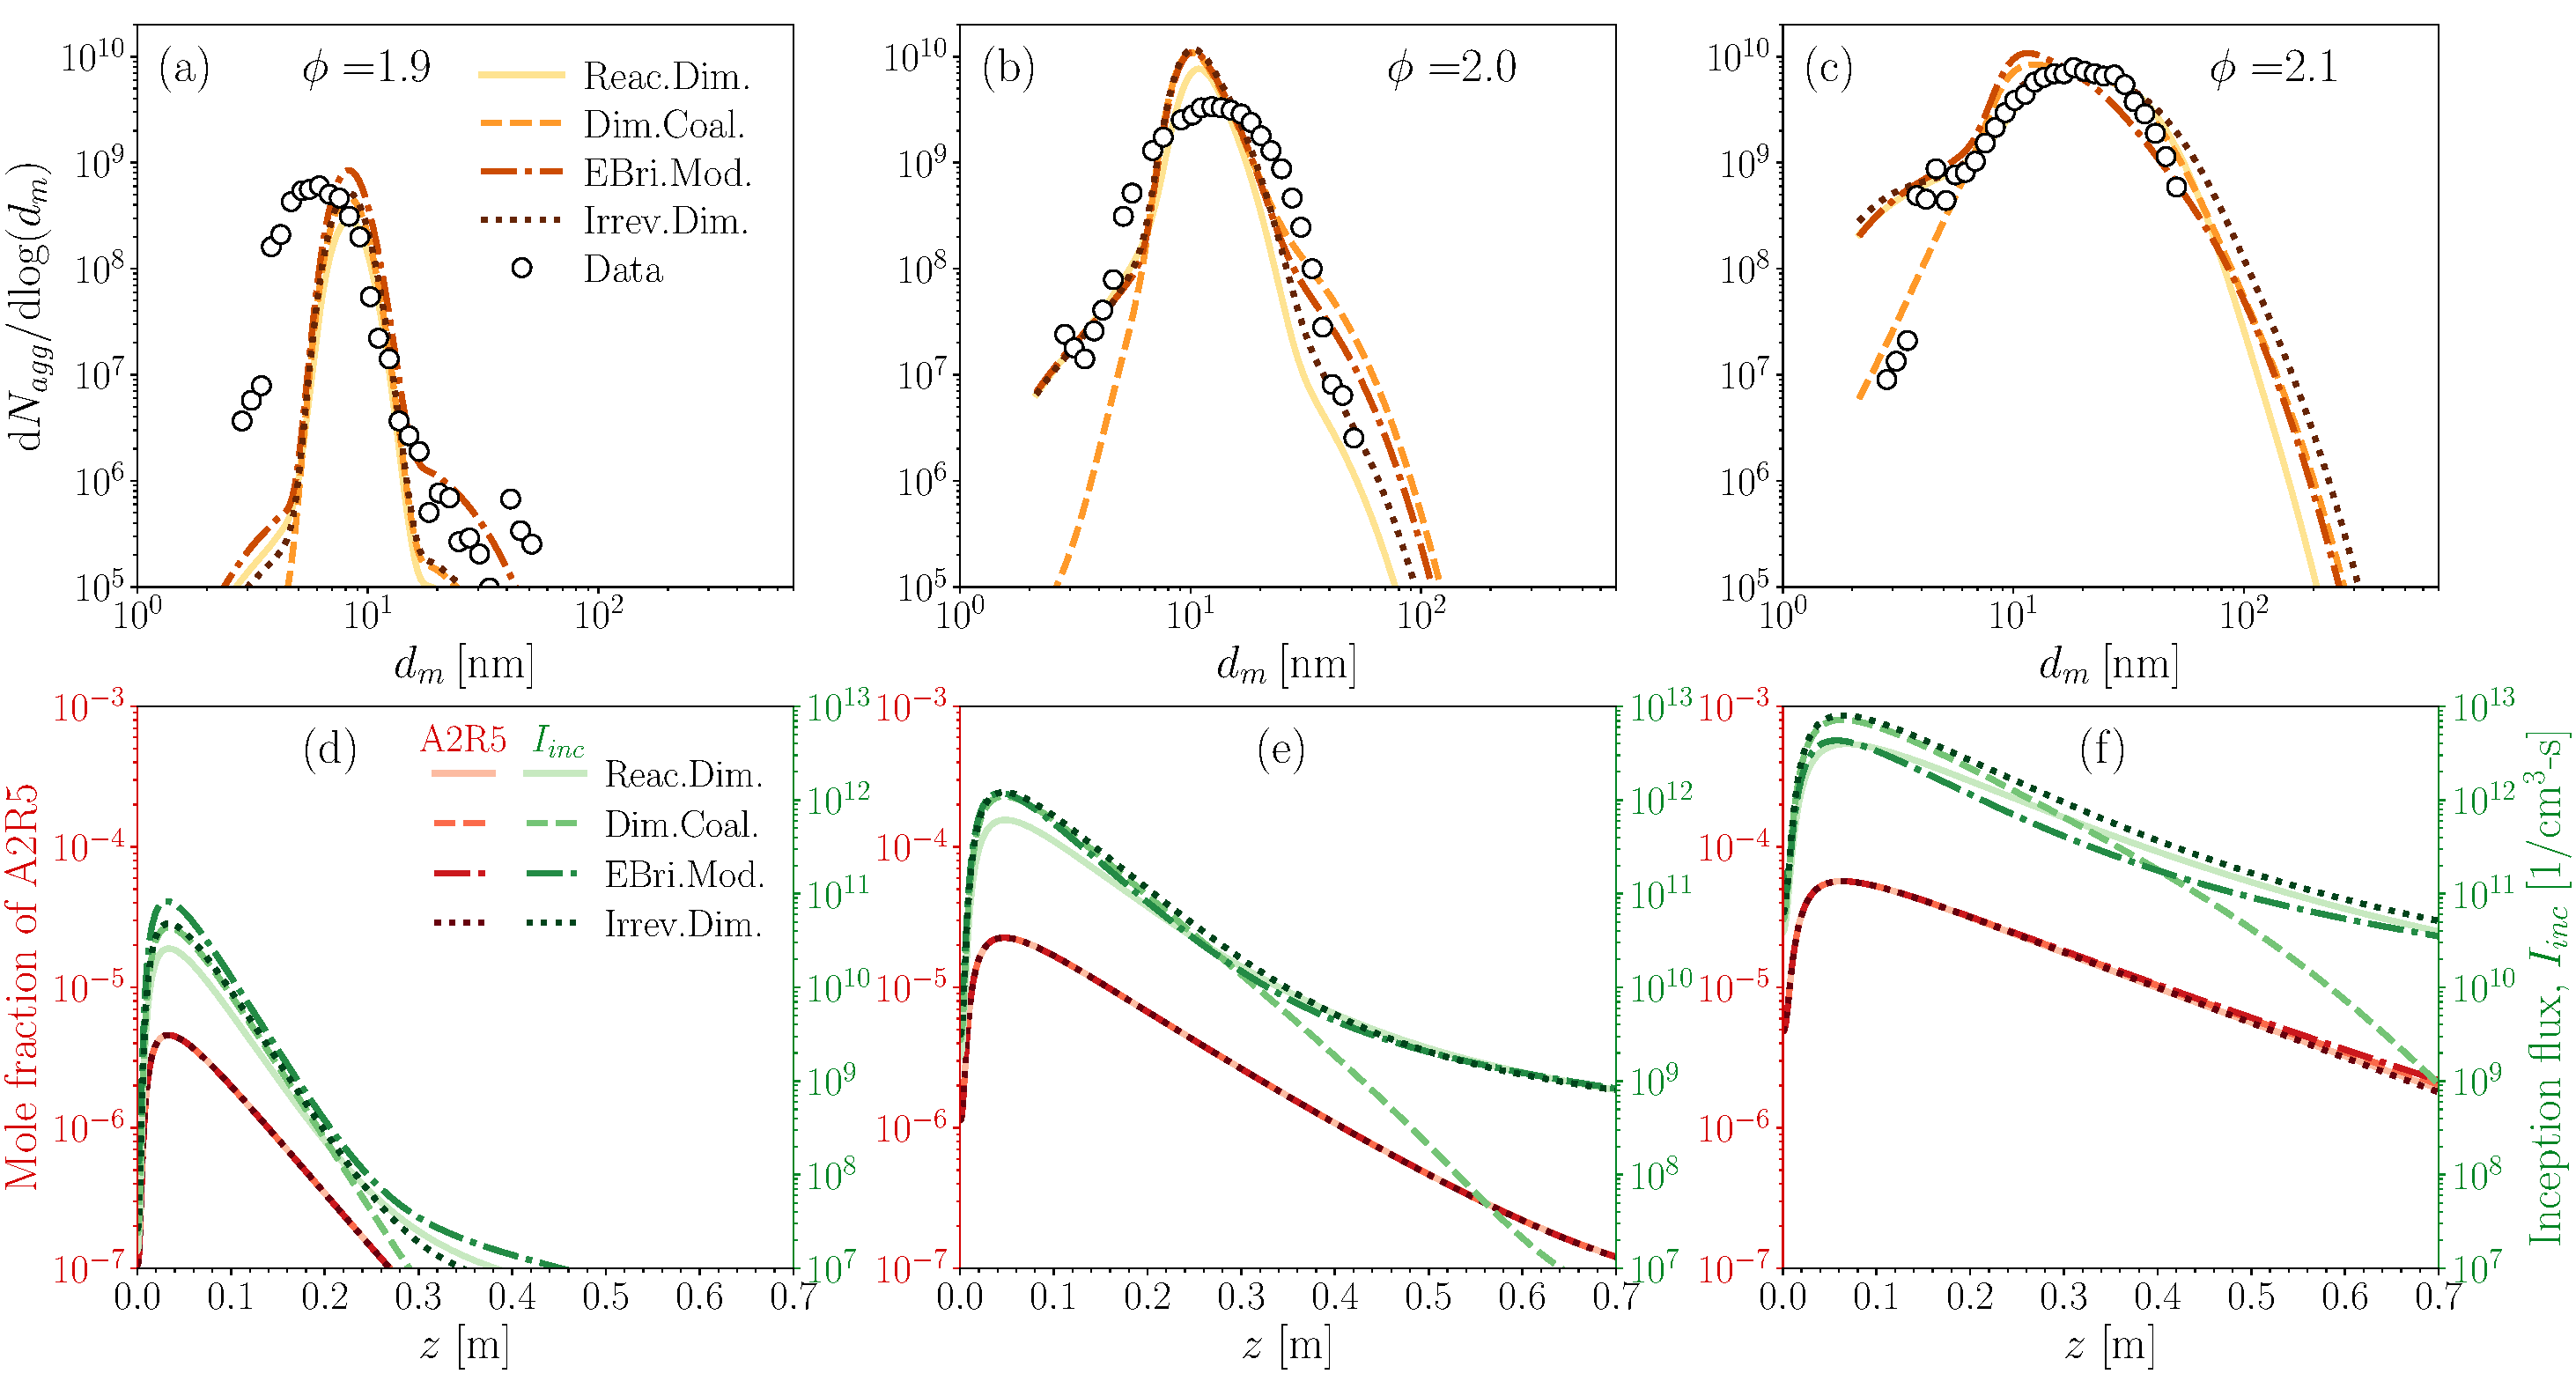
\includegraphics[width=1\textwidth]{Figures/Results/Paper1/PSR/PSD_eq_ratio_log.pdf}};
		\draw (-3.85, 2.75) node {\scriptsize{\cite{manzello2007soot}}};
		%\draw (1.95, 0.66) node {\tiny{\cite{manzello2007soot}}};
		%\draw (5.5, -1.28) node {\tiny{\cite{manzello2007soot}}};
	\end{tikzpicture}
	\caption{The particle size distribution at the end of PFR, and the mole fraction of A2R5, and inception flux, $I_{inc}$ along the PFR for $\phi=1.9$ (a, d), 2.0 (b, e), and 2.1 (c, f) obtained using KAUST mechanism, SPBM and different inception models calibrated to match the predictions with the PSD measurements~\citep{manzello2007soot}.}
	\label{fig:psrpfr_psd} 
\end{figure*}


The KAUST mechanism was used to describe the gas-phase chemistry. The inception and PAH adsorption adjustment factors were varied for each PAH growth model to match the predicted PSD with the measurements as closely as possible for all three equivalence ratios. A similar match could not be reached using the Caltech mechanism because the number concentration of particles was underestimated by at least four orders of magnitude even with $\eta_{inc}=\eta_{ads}=1$. Table~\ref{tab:adjustfactor_psr} lists the adjustment factors used with the KAUST mechanism for simulations of ethylene oxidation in the studied perfectly stirred reactor.

\begin{table}[!t]
	\caption{The value of adjustment factors used in the simulation of ethylene oxidation in the perfectly stirred reactor.}
	\label{tab:adjustfactor_psr}
	\centering
	\begin{tabular}{lllll}
		\hline
		& Reac.Dim. & Dim.Coal. & EBri.Mod. & Irrev.Dim. \\
		\hline
		$\eta_{inc}$ & 0.0005     & 0.001      & 0.0002       & 0.01        \\
		$\eta_{ads}$ & 0.01      & 0.01      & 0.01       & 1 \\
		\hline       
	\end{tabular}
\end{table}

As shown in Fig.~\ref{fig:psrpfr_psd}, all inception models capture the peak number concentration and the unimodal shape of the PSD, indicating that particle inception has ceased and coagulation is the dominant mechanism for agglomerate size growth. As reported in Table~\ref{tab:psrpfr_morpcomp}, the geometric mean mobility diameter, $d_{m,g}$, and the geometric mobility standard deviation, $\sigma_{m,g}$, obtained using all inception models are in good agreement with the values calculated from the measured PSD~\citep{manzello2007soot}. As shown in Fig.~\ref{fig:psrpfr_psd}a-b, the spread of the predicted PSD is narrower than that of the measurements for $\phi = 1.9$ and 2.0, corresponding to an underprediction of $\sigma_{m,g}$ for these equivalence ratios.

\begin{table}[H]
	\centering
	\caption{The geometric mean mobility diameter, $d_{m,g}$, and the geometric mobility standard deviation, $\sigma_{m,g}$, obtained using different inception models compared with the value calculated from the measured PSD~\citep{manzello2007soot}.}
	\label{tab:psrpfr_morpcomp}
	%\begin{tabular}{l|ll|ll|ll|}
	\begin{tabular}{lllllll}
		\cline{2-7}
		& \multicolumn{2}{c}{$\phi=1.9$}                   & \multicolumn{2}{c}{$\phi=2.0$} & \multicolumn{2}{c}{$\phi=2.1$} \\ \cline{2-7} 
		& \multicolumn{1}{l} {$d_{m,g}$  [nm]} & $\sigma_{m,g}$ & \multicolumn{1}{l} {$d_{m,g}$  [nm]} &  $\sigma_{m,g}$ & \multicolumn{1}{l}{$d_{m,g}$  [nm]} & $\sigma_{m,g}$ \\ \hline
		\multicolumn{1}{l}{\textbf{Data}~\citep{manzello2007soot}}                      & \multicolumn{1}{l}{\textbf{6.04}}          &     \textbf{1.25}      & \multicolumn{1}{l}{\textbf{12.40}} &  \textbf{1.49} & \multicolumn{1}{l}{\textbf{17.66}} & \textbf{1.64} \\ %\hline
		\multicolumn{1}{l}{Reactive Dimerization}     & \multicolumn{1}{l}{8.27}          &    1.14       & \multicolumn{1}{l}{11.10} & 1.21  & \multicolumn{1}{l}{16.88} & 1.58  \\ %\hline
		\multicolumn{1}{l}{Dimer Coalescence}         & \multicolumn{1}{l}{8.18}          &      1.14     & \multicolumn{1}{l}{10.76} & 1.24 & \multicolumn{1}{l}{16.99} & 1.68 \\ %\hline
		\multicolumn{1}{l}{E-Bridge Modified}          & \multicolumn{1}{l}{8.27}          &    1.15       & \multicolumn{1}{l}{11.02} & 1.27 & \multicolumn{1}{l}{14.56} & 1.58 \\ %\hline
		\multicolumn{1}{l}{Irreversible Dimerization} & \multicolumn{1}{l}{8.19}          &      1.14     & \multicolumn{1}{l}{10.96} & 1.25 & \multicolumn{1}{l}{18.44} & 1.78 \\ \hline
	\end{tabular}
\end{table}


All inception models underpredict the number concentration of small particles ($d_m < 6$~nm) at $\phi = 1.9$. The discrepancy decreases at $\phi = 2.0$, and the model predictions align well with the measurements except for Dimer Coalescence model that underpredicts the number concentration of small particles ($d_m<5$~nm). In the simulation results, the number concentration of the smallest particles with a diameter of 2~nm is strongly affected by the equivalence ratio, as the precursor production rate increases with $\phi$. This behavior can be better understood by comparing the acenaphthylene (A2R5) mole fraction at different $\phi$ values, as shown in Fig.~\ref{fig:psrpfr_psd}d-f. The inlet mole fraction of A2R5 at $z = 0$~m corresponds to the value obtained from the PSR, which increases by factors of 10 and 4 when $\phi$ is increased incrementally from 1.9 to 2.0, and from 2.0 to 2.1, respectively. This relative increase is nearly the same across all inception models. The jump in A2R5 mole fraction leads to a substantial increase in the inception flux, which explains the sensitivity of the smallest particle concentrations to the equivalence ratio. The strong similarity between the A2R5 mole fraction profiles and the soot inception profiles along the reactor highlights the dominant role of A2R5 in soot inception. Another important observation is that the A2R5 mole fraction is not affected by the choice of inception model.


As shown in Fig.~\ref{fig:psrpfr_fv}a-c, $d_p$ along the PFR is nearly identical for all inception models at $\phi = 1.9$, but the differences become more noticeable at higher $\phi$ values. The Reactive Dimerization model predicts the largest final $d_p$ because it channels more PAH mass into PAH adsorption rather than inception, which is consistent with the lower peak number concentration observed in Fig.~\ref{fig:psrpfr_psd}. The value of $d_p$ decreases rapidly at the beginning of the reactor due to a surge in the production of incipient particles (spherical particles with a diameter of 2~nm), which lowers the mean $d_p$. It then increases toward the end of the reactor as surface growth becomes dominant. Although the final $d_p$ increases slightly with $\phi$, the overall range remains similar across $\phi$ values, indicating a comparable balance between inception and surface growth. 

\begin{figure*}[!t]
	\centering
	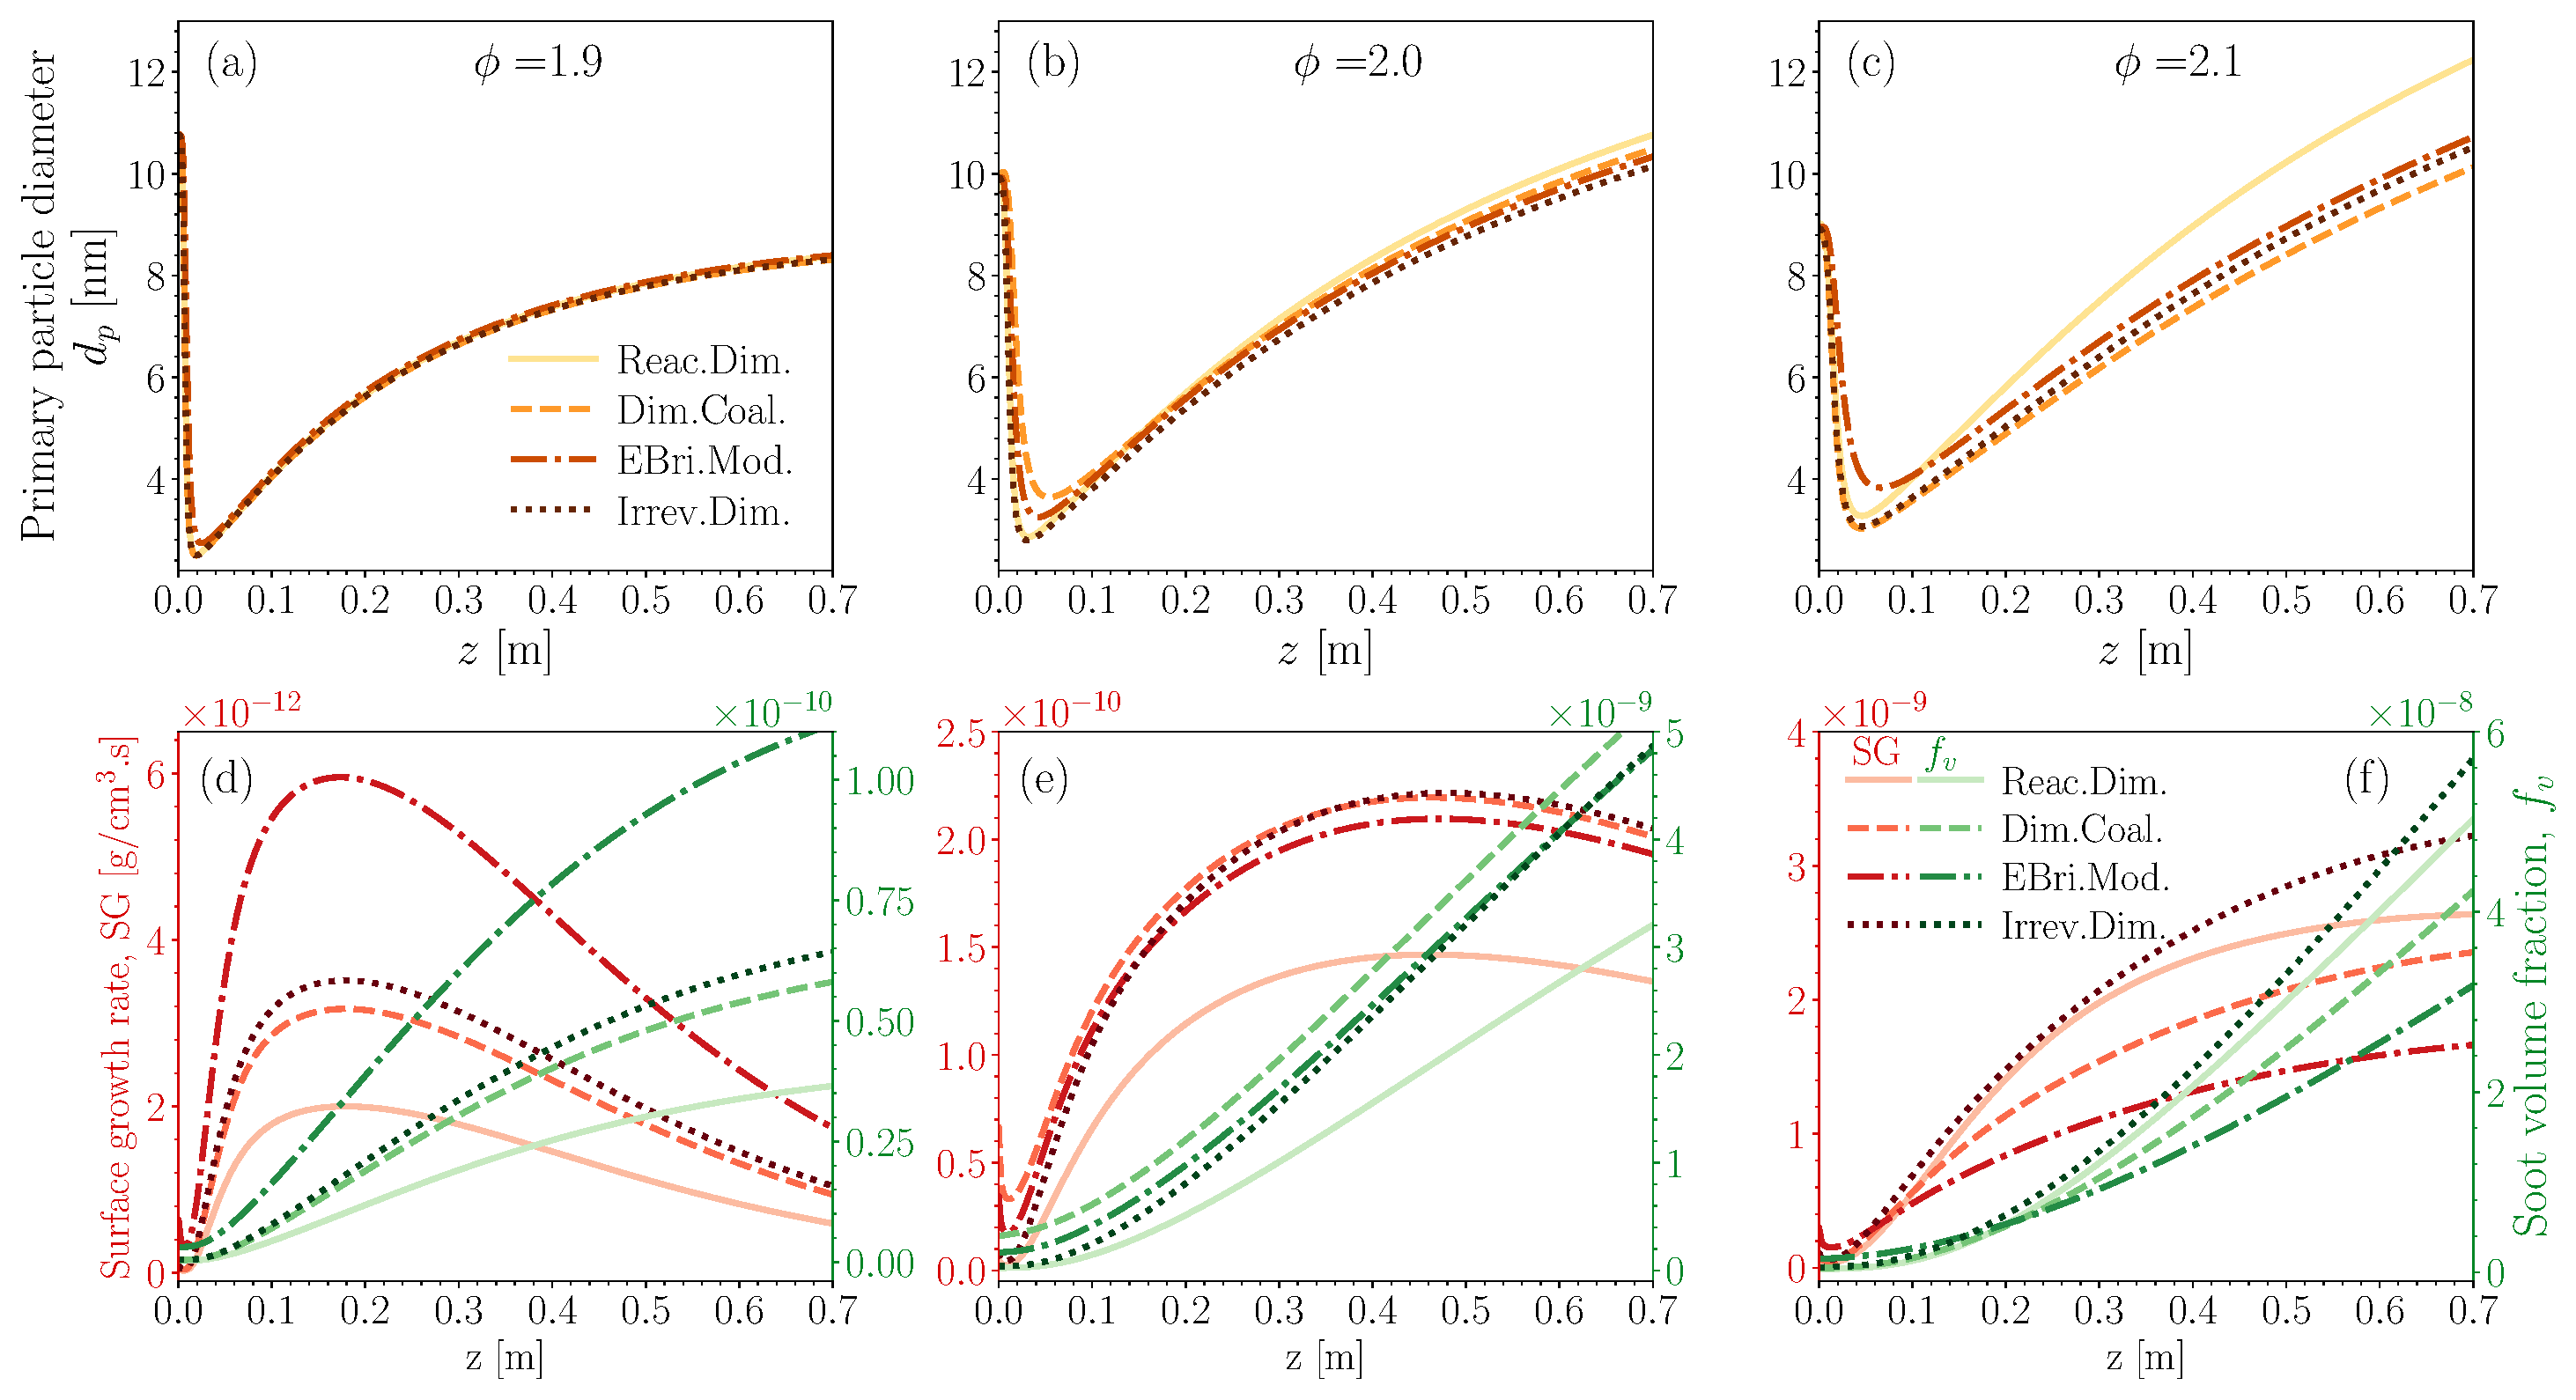
\includegraphics[width=1\textwidth]{Figures/Results/Paper1/PSR/surface_growth_fv.pdf}
	\caption{The primary particle diameter, $d_p$, the total surface growth rate by HACA and PAH adsorption, and the soot volume fraction, $f_{v}$ along the PFR for $\phi=1.9$ (a, d), 2.0 (b, e), and 2.1 (c, f) obtained using KAUST mechanism, SPBM and different inception models calibrated to match the predictions with the PSD measurements~\citep{manzello2007soot}.}
	\label{fig:psrpfr_fv} 
\end{figure*}

As shown in Fig.~\ref{fig:psrpfr_fv}, the surface growth rate (HACA and PAH adsorption combined) and the soot volume fraction, however, are highly sensitive to $\phi$, which can be attributed to the strong influence of $\phi$ on precursor production, inception flux, and the number of particles. An analysis of surface growth rates at the end of the PFR revealed that more than 95\% of the soot mass is acquired through the HACA mechanism. The apparent difference in $f_v$ between the inception models originates from the different PAH adsorption rate predicted by the inception models. For example, at $\phi = 1.9$, the E-Bridge Modified model predicts the highest surface growth rate and soot volume fraction due to a higher number of agglomerates (as shown in Fig.~\ref{fig:psrpfr_psd}a), which leads to a larger total surface area, which is the key factor in calculating the HACA growth rate.




